\section{Ideas preliminares}
Considere un experimento aleatorio y suponga que evoluciona o cambia de un estado a otro a lo largo del tiempo y sea $X_t$ el estado del experimento al tiempo $t$, de tal forma que cada $X_t$ es una variable aleatoria para cada $t$. Esta colección de variables aleatorias se conoce como proceso estocástico, y sirve como modelo para representar la evolución aleatoria de un sistema a lo largo del tiempo.\\
Las demostraciones de los resultados expuestos en este capítulo se pueden encontrar en \cite{Feller}, \cite{Rincon3} \\
\begin{Def}
    Un proceso estocástico de define como una colección de variables aleatorias $\{X_t\}_{t\in T}$ definidas en algún espacio de probabilidad $(\Omega,\thinspace\mathscr{F})$, que es parametrizada por un conjunto $T$ ( el cual es llamado espacio parametral), en donde las variables aleatorias toman valores en un conjunto $S$ denominado espacio de estados.
\end{Def}
Un proceso estocástico puede interpretarse como una sucesión de variables aleatorias cuyas características pueden variar a lo largo del tiempo.
Puede tenerse un espacio de estado discreto o un espacio de estado continuo. En el caso más simple, se utiliza un conjunto discreto como espacio de parámetros $T= \{0, 1, 2,\ldots\}$ y estos números se interpretan como tiempos épocas. En este caso se dice que el proceso es a tiempo discreto (también conocido como cadenas), este tipo
de procesos será denotado en general por $\{X_n\}^{\infty}_{n=0}$, o $\{X_n:\thinspace n= 0, 1, \ldots\}$ dependiendo de la complejidad de la notación de la variable aleatoria a utilizar.\\Por lo tanto para cada $n$, se tiene que $X_n$ vendría a ser el valor del proceso o estado del sistema al tiempo $n$.
Se puede tomar como ejemplo a los cambios que podrían ocurrir "cada día, cada mes, cada año, etc."\\ En el caso del tiempo continuo, el espacio parametral se considera como el conjunto continuo $T=[0,+\infty)$ donde los cambios de estado se podrían realizar en cualquier instante.\\
A partir de ahora, seguiremos la convención de si el subíndice de la variable aleatoria es denotada con $n$, entonces el espacio parametral será discreta, mientras que si el subíndice es $t$, el tiempo se medirá de manera continua.\\
\begin{Ejm}
    Considere una máquina en una fábrica. Un posible estado de la máquina es si está funcionando o no, esta verificación se realiza al comienzo de cada día hábil. Se le asigna el estado "inactivo" a un valor de $0$ y el estado "activo" a un valor de $1$. Una colección de variables aleatorias es proporcionada por.
    $$X_t=
    \label{ejm-procEstocástico}
    \begin{cases}
        0, & \mbox{Si la máquina está 'inactivo' en el tiempo $t$}\\
        1, & \mbox{Si la máquina está 'activo' en el tiempo $t$}
    \end{cases}$$
    La figura (\ref{fig-procesoEstocástico-Ejemplo}) muestra una posible secuencia de cambios de estado a través del tiempo para esa máquina.
    \begin{center}
        \begin{figure}[htb]
            \begin{center}
             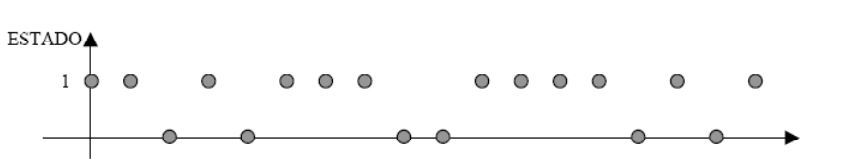
\includegraphics[width=14cm]{Cap2-ProcesosEstocásticos/img/ejem1.JPG}
                \vspace*{0.05in}
            \end{center}
            \caption{Estado que se encuentra la máquina al tiempo $t$ }
            \label{fig-procesoEstocástico-Ejemplo}
        \end{figure}
    \end{center}
    Según la gráfica, la máquina al tiempo $0$ y $1$ se encuentra en operación, por eso:
    $$X_0=1$$
    $$X_1=1$$
    Al tiempo $2$ la máquina cambia de estado y se encuentra fuera de funcionamiento. 
    $$X_2=0$$
   Sucesivamente vemos como la máquina va cambiando de estado constantemente a través del tiempo.
    $$X_3=1$$
    $$X_4=0$$
    $$\vdots$$
\end{Ejm}
\begin{Obs}
Para cualquier $t\in T$ se denota $P(X(t)=i)$, $P_t=i$ o $P(X_t=i)$ como la probabilidad que en el tiempo $t$ el ensayo está en el estado $i$, es decir $P(\omega\in\Omega,\thinspace X_t(\omega)=i).$
\end{Obs}
Un proceso estocástico, también llamado proceso aleatorio, puede considerarse como una función de dos variables
$$X:T\times\Omega\rightarrow S$$ a la cual a cada $(t,\thinspace\omega)$ se le asocia el valor o estado $X (t,\thinspace\omega) $.\\
Para cada valor aleatorio $t$ en $T$ , el mapeo $X_t$ , $X_t: \Omega\rightarrow S$ es una variable aleatoria, mientras que para cada $\omega$ en $\Omega$ fijo arbitrario, la función $X(\cdot\thinspace,\thinspace\omega)$ es llamada una trayectoria.\\En este trabajo estaremos interesados en el caso de procesos estocásticos con espacio de estados discreto, suele representarse de la siguiente
manera: $$(X_0=k_0,\thinspace\ldots,\thinspace X_n=k_n)$$
La principal preocupación de los estudios realizados en casos discretos es calcular la probabilidad de ocupación de cada estado a partir de la probabilidad particular de cambio de estado. ¿Con qué probabilidad se estará en el estado $k_n$ en el instante $n$ dado que en el instante $n-1$ el proceso se encontraba en el estado $k_{n-1}$? Esta probabilidad de denotará como:
$$P(X_n = k_n\mid X_{n-1} = k_{n-1})$$
A este tipo de probabilidad condicionada se le denomina probabilidad de transición o de cambio de estado. $P(X_n = k_n\mid X_{n-1} = k_{n-1})$. \\Otra forma de denotarlo es $P(X_n = k_n \mid X_{n-1} := k_{n-1})=P_{i j}{(n-1,n)}$
\begin{Ejm}
    Del proceso estocástico expuesto en el ejemplo (\ref{ejm-procEstocástico}), \\$P_{0,1}(n-1,n)=P(X_n=1\mid X_{n-1}=0)$ denota la probabilidad de que en el tiempo $n$ la máquina esté 'en operación' , dado que previamente en el tiempo $n-1$ se encontraría 'fuera de funcionamiento'.\\
    $P_{1,0}(n-1,n)=P(X_{n-1}=0\mid X_n=1)$ denota la probabilidad de que en el tiempo $n$ la máquina se encuentre 'fuera de funcionamiento', dado que previamente en el tiempo $n-1$ estaba 'en operación'.\\
    $P_{0,0}(n-1,n)=P(X_{n-1}=0\mid X_n=0)$ denota la probabilidad de que en el tiempo $n$ la máquina esté 'fuera de funcionamiento', dado que previamente en el tiempo $n-1$ también se encontraba 'fuera de funcionamiento'.
\end{Ejm}
Una propiedad interesante que se presentan en algunas cadenas es que los valores de sus probabilidades de transición no dependan del valor de $n$. Es decir, "las probabilidades de cambiar de estado son las mismas en cualquier instante y no dependen del tiempo en que se encuentre el experimento, más bien lo relevante es el tiempo que transcurre durante la transición de estados". Esto es $$P_{i j}(0,n)=P_{i,j}(k,k+n),\quad \forall k\in\N$$.\\
A este tipo de transiciones se le conoce como estacionarias y se denotan por simplicidad $P_{i,j}(n)$, en vez de $P_{i,j}(k,k+n)$ para cualquier $k\in T$, de esta manera se resalta que el tiempo transcurrido es $n$.\\
\begin{Obs}
    Sea $P_{i,j}(m,n)$ una probabilidad de transición estacionaria arbitraria. Por definición tenemos que $P_{i,j}(m,n)=P_{i,j}(n-m)$
\end{Obs}
\begin{Def}
    Sea  $\{X_t\}_{t\in T}$ un proceso estocástico con valores en el conjunto de estados $S=\{x_0,\thinspace x_1,\thinspace x_2 ,\ldots\}$ ( S puede ser finito o numerable ).
    Decimos que $\{X_t\}_{t\in T}$ es una cadena de Markov si cumple la siguiente propiedad conocida como la condición de Markov
    \begin{eqnarray}
    P(X_{n+1}=k_{n+1}\mid  X_{0}=k_0,\thinspace\ldots,\thinspace X_{n}=k_n)=P(X_{n+1}=k_{n+1}\mid X_{n}=k_n)
    \label{procesosEstocásticos-condMarkov}
    \end{eqnarray}
    Esto significa que la probabilidad de que el suceso $k_{n+1}$ ocurra en el tiempo $n+1$ (futuro) solo dependerá de la ocurrencia del evento $k_n$ en el tiempo $n$ (presente), mientras que la información de lo que ocurrió en los tiempos $0,\thinspace 1,\thinspace 2, \ldots,n-1$ (pasado) es irrelevante.
\end{Def}
\begin{Teo}
    La condición de Markov (\ref{procesosEstocásticos-condMarkov}) es equivalente a poder calcular la distribución conjunta de las variables $\{X_k\}_{k=1}^n$ de la siguiente forma:
    \begin{eqnarray}
    \label{procesosEstocásticos-condMarkovEquiv}
    P(X_0= k_0,\thinspace\ldots,X_{n+1}= k_{n+1}) =P(X_0=k_0)P(X_1=k_1|\thinspace X_0=k_0)\cdots P(X_{n+1}=k_{n+1}|\thinspace X_n=k_n)
    \end{eqnarray}
\end{Teo}
Puede considerarse que la denominada cadena de Markov inicia su evolución iniciando en un estado $i$ cualquiera, o de manera más generalizada considerando una
distribución de probabilidad inicial sobre un espacio de estados. Una distribución inicial para una cadena de Markov con espacio de estados $t= 0, 1,\thinspace 2,\thinspace,\ldots  $ es simplemente una distribución de probabilidad sobre este conjunto, es decir,
es un conjunto de números $p_0,\thinspace p_1,\thinspace p_2 ,\ldots >0$ cuya suma converge a uno. El número $p_i$ corresponde a la probabilidad de que la cadena inicie en el estado $i$, es decir $P(X_0= i)$\\ \\
\begin{Obs}
    En las cadenas de Markov en tiempo discreto, utilizamos como índice un tiempo
    discreto $n=0, 1, 2,\ldots$ y se deducían numerosas propiedades.
    Las nociones de cadenas de Markov se puede extender a un tiempo continuo $t \geq 0$.
\end{Obs}
Consideremos un proceso a tiempo continuo $\{X_t\}_{t\geq 0}$ que inicia en un estado $i_1$.
\begin{figure}
    \centering
    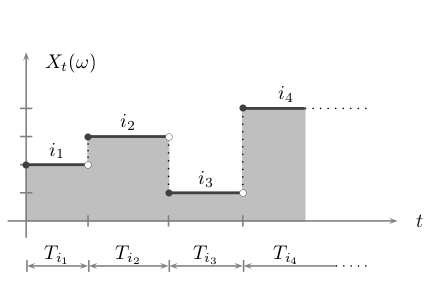
\includegraphics[width=10cm]{Cap2-ProcesosEstocásticos/img/procesos_continuos.png}
    \caption{Proceso estocástico a tiempo continuo}
    \label{fig-procEstocastContinuo}
\end{figure}
El proceso permanece en ese estado un tiempo $T_{i 1}$ y
después toma el valor de un nuevo estado $i_2$ distinto del anterior, permanece en ese estado un tiempo determinado $T_{i 2}$ hasta llegar a un estado posterior y así sucesivamente. Esta
sucesión de saltos se muestra gráficamente en la figura \ref{fig-procEstocastContinuo}
Los tiempos aleatorios $T_{i_j}$ son aquellos
en los que el proceso permanece constante en alguno de sus estados, son denominados tiempos de estancia.
Los momentos en donde el proceso cuenta con "saltos" son los tiempos $W_n=T_{i_1}+\cdots+T_{i_n}$ $n\in\N$.
Nuestro proceso estocástico $\{X_t\}_{t\geq 0}$ puede ser descrito como:
 $$X_t =
 \begin{cases}
    i_1, & \mbox{ Si $0\leq t <W_1$}\\
    i_2, & \mbox{ Si $0\leq t <W_2$}\\
    i_3, & \mbox{ Si $0\leq t <W_3$}\\
    \vdots
 \end{cases}$$
\begin{Def}
    Sea $\{X_t\}_{t\geq 0}$ un proceso estocástico sobre el conjunto de estados $S$, es una cadena de Markov de tiempo continuo si $S$ es numerable y para cualquier $0\leq t_1<t_2<\ldots<t_n<t_{n+1}$ se tiene  $$P\big(X_{t_n}=i_n\mid X_{t_1}=i_{t_1},\ldots ,\thinspace X_{t_{n-1}}=i_{t_{n-1}}\thinspace \big)=P\big(X_{t_n}=i_n\mid X_{t_{n-1}}=i_{t_{n-1}}\big)$$
\end{Def}
Observe que no estamos suponiendo el conocimiento de la historia previa del suceso, si no, únicamente en una colección finita arbitraria de tiempos pasados $t_1,t_2,t_3,\ldots,t_{n-1}$.\\
Supondremos nuevamente que estas probabilidades de transición son estacionarias en el tiempo (para cada $s\leq 0$ y $t\leq 0$, la probabilidad $P(X_{t+s} =j \mid X_s= i)$ 
es idéntica a $P(X _{t} =j \mid X_0= i)$), esta probabilidad se denota mediante la expresión $P_{i j}(t)$, para $i$ y $j$ enteros no negativos.\\
\begin{Obs}
    En particular para $t= 0$, tanto para el caso continuo como discreto, se define la probabilidad de transición $P_{i j}(0)$ como la función delta de Kronecker, es decir,
    $$P_{i,j}(0)=\delta_{i j}=\begin{cases}
        1, & \mbox{Si $i=j$}\\
        0, & \mbox{Si $i\not= j$}
    \end{cases}$$
    Esto nos da a entender que, cuando el tiempo aún no transcurre ( se encuentra en la etapa inicial ), la probabilidad de que ocurra un cambio es nula, mientras que la probabilidad de que permanezca en el mismo estado ( que no cambie ) es absoluta, es decir $1$.
\end{Obs}
Cuando los índices $i$ y $j$ varían, por ejemplo, sobre el conjunto de estados $t=\{ 1,\thinspace 2,\ldots, n\}$ , se le conoce como matriz de probabilidades de transición de paso $t$, $t\geq 0$
$$P(t)=\left( \begin{array}{ccc}
p_{0 0}(t) & \cdots & p_{0 n}(t) \\ 
p_{1 0}(t) & \cdots & p_{1 n}(t)\\
\vdots & \ddots & \vdots \\
p_{n 0}(t) & \cdots & p_{n n}(t) 
\end{array}\right)\\$$
\begin{Ejm}
    En Perú existen $3$ operadores principales de telefonía móvil como lo son Movistar, Claro y Entel (estados).
    Los porcentajes actuales que tiene cada operador en el mercado actual son para Movistar $0.4$ para Claro $0.25$ y para Entel $0.35$. (estado inicial).
    Un usuario de Movistar actual tiene una probabilidad de permanecer en Movistar de $0.60$, una probabilidad de cambiar a Claro de $0.2$ y la probabilidad de pasarse a Entel de $0.2$.\\Por otro lado, si el usuario es cliente de Claro tiene una probabilidad de mantenerse en Claro del $0.5$, de que esta persona se cambie a Movistar  $0.3$ y que se pase a Entel de $0.2$.\\Y si el usuario es cliente de Entel la probabilidad que permanezca es de $0.4$, de que se cambie a Movistar de $0.3$ y a Claro de $0.3$.\\
    Nuestra proceso estocástico estaría dado por $\{X_t\}_{t\leq 0}$ donde para dado tiempo $t\geq 0$, $\thinspace X_t(Movistar)=0$ ,$\thinspace X_t(Claro)=1$, $\thinspace X_t(Entel)=2$, partiendo de esta información podemos elaborar la matriz de transición.
   $$P(1)=\left( \begin{array}{ccc}
    P_{0 0}(1) & P_{0 1}(1) & P_{0 2}(1) \\
    P_{1 0}(1) & P_{1 1}(1) & P_{1 2}(1) \\
    P_{2 0}(1) & P_{2 1}(1) & P_{2 2}(1)  
    \end{array}\right)=
    \left( \begin{array}{ccc}
    0.60 & 0.2 & 0.2 \\ 
    0.3 & 0.5 & 0.2 \\
    0.3 & 0.3 & 0.4
    \end{array}\right)\\$$
    La suma de las probabilidades de cada estado (en este caso el operador telefónico) deben ser iguales a $1$. Nuestro estado inicial en este caso sería $$P(X_0 = 0)= 0.4,\thinspace P(X_0 = 1)= 0.25 ,\thinspace P(X_0 = 2)= 0.35$$
    Para descubrir el valor de la probabilidad de una persona usando Movistar en la época $0$ y luego empiece a usar Claro en la época $1$. 
    $$P(X_1=1 , X_0=0) = P(X_0=0)P_{01}(1)= 0.40\cdot 0.20 =0.08$$
    Para descubrir el valor de la probabilidad de que una persona use Entel en la época $0$ y luego empiece a usar Movistar en la época $1$ está dado por
    $$P(X_1=0 , X_0=2) = P(X_0=2)P_{20}(1)=0.35\cdot 0.3 =0.105$$
    y si suponemos que nuestro proceso estocástico cumple la condición de Markov (\ref{procesosEstocásticos-condMarkov}) de pérdida de memoria, (no nos importa qu\'e operador us\'o  mucho antes, solo nos interesa el operador usado previamente antes de la transición) entonces para calcular, por ejemplo la probabilidad de que una persona use Movistar en la época $0$, luego use Claro en la época $1$ y finalmente Entel en la época $2$ usamos la condición equivalente (\ref{procesosEstocásticos-condMarkovEquiv}).
    $$P(X_2=2,\thinspace X_1=1,\thinspace X_0=0)=P(X_0=0)P_{01}(1)P_{12}(1)=0.4\cdot 0.2\cdot 0.2=0.016$$
    \end{Ejm}
    De esta forma encontramos que la probabilidad de que una persona elija Movistar y luego se cambie de operador a Movistar y finalmente acabe usando Entel es $0.016$.
\begin{comment}
    \begin{Teo}(Ecuación de Chapman-Kolmogorov)
        Para cualquier
        par de números enteros $m$ y $n$ tales que $0\leq m\leq n$, y para cualesquiera estados $i$ y $j$ se cumple
        \begin{eqnarray}
            p_{i,j}(m,n)=\sum_k p_{i,k}(m,u)P(u,t)
        \end{eqnarray}
    \end{Teo}
\end{comment}